\documentclass[11pt]{standalone}
\usepackage{amssymb}
\usepackage{amsmath}
\usepackage[no-math]{fontspec}
\usepackage{unicode-math}
\usepackage{libertinus}
\usepackage{pgf,xcolor}
\usepackage{tikz}
\usetikzlibrary{arrows.meta, backgrounds}
\usepackage{pgfplots}
\pgfplotsset{compat=newest}

\setmainfont{Libertinus Serif}
\setmathfont{Libertinus Math}

\definecolor{my_darkgray}{HTML}{484949}
\definecolor{my_lightgray}{HTML}{F3F4F4}
\definecolor{my_darkblue}{HTML}{005A94}
\definecolor{my_lightblue}{HTML}{CCDEE9}
\definecolor{my_yellow}{HTML}{FFEC7F}
\definecolor{my_red}{HTML}{E60000}
\definecolor{my_orange}{HTML}{E87846}

\begin{document}

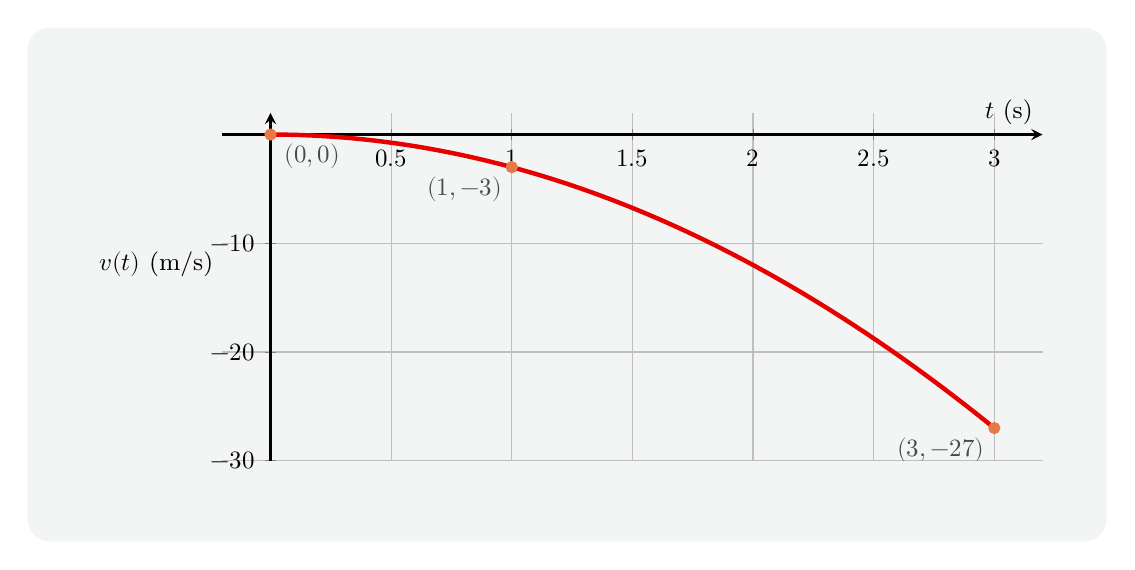
\begin{tikzpicture}[
    show background rectangle,
    background rectangle/.style={fill=my_lightgray, rounded corners=8pt},
    inner frame sep=0.8cm
]

\begin{axis}[
    width=12cm,
    height=6cm,
    axis lines = center,
    xlabel = {$t$ (s)},
    ylabel = {$v(t)$ (m/s)},
    xmin=-0.2, xmax=3.2,
    ymin=-30, ymax=2,
    grid = both,
    axis line style={thick},
    ticklabel style={font=\small},
    label style={font=\small},
    ylabel style={
      at={(axis description cs:-0.08,0.5)},
      anchor=south
    },
]

% velocity profile v(t) = -3 t^2 on [0, 3]
\addplot[
    draw=my_red,
    ultra thick,
    samples=300,
    domain=0:3
]
{-3*x^2};

% mark summit velocity at t = 0: (0, 0)
\addplot[
    only marks,
    mark=*,
    mark size=2pt,
    draw=my_orange,
    fill=my_orange
]
coordinates {(0,0)};

\node[anchor=north west, font=\small, my_darkgray]
at (axis cs:0,0) {$\,(0, 0)$};

% mark velocity at t = 1: (1, -3)
\addplot[
    only marks,
    mark=*,
    mark size=2pt,
    draw=my_orange,
    fill=my_orange
]
coordinates {(1,-3)};

\node[anchor=north east, font=\small, my_darkgray]
at (axis cs:1,-3) {$(1, -3)$};

% mark velocity at t = 3: (3, -27)
\addplot[
    only marks,
    mark=*,
    mark size=2pt,
    draw=my_orange,
    fill=my_orange
]
coordinates {(3,-27)};

\node[anchor=north east, font=\small, my_darkgray]
at (axis cs:3,-27) {$(3, -27)$};

\node[anchor=south west, font=\small\bfseries, my_darkgray]
at (rel axis cs:0.02,0.98)
{Velocity $v(t) = s'(t) = -3t^2$ during the first descent};

\end{axis}

\end{tikzpicture}

\end{document}